\begin{figure}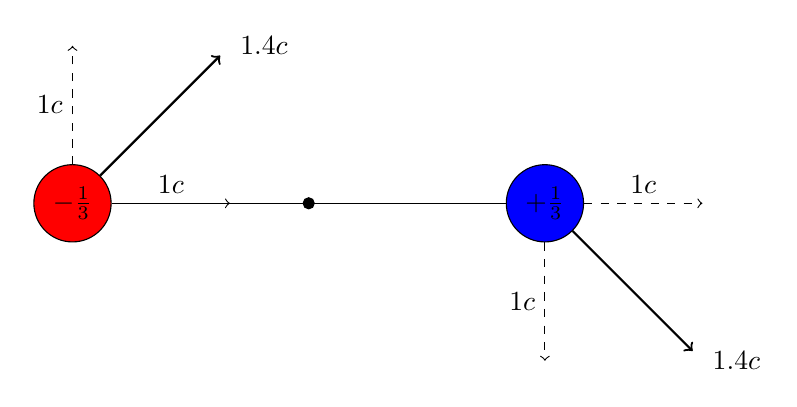
\begin{tikzpicture}[scale=1, rotate=0]


% photon horizontal with speed vectors



\path 
(0,0) node[circle,draw, fill=red](red) {$-\frac{1}{3}$}
(6,0) node[circle,draw, fill=blue](blue) {$+\frac{1}{3}$};
\draw[black] (red) -- (blue)          node[pos=0.5](center){};
\filldraw
 (center) circle (2pt);
%\draw[->, black] (center) -- ++(1,0) node [anchor=west]{};

%% Arrows indicating the speed components from blue
\draw[->, black, dashed] (blue) -- node[above] { $1c$} ++(2,0) node [](west){};
\draw[->, black, dashed] (blue) -- node[left] { $1c$} ++(0,-2) node [](south){};
\path (west) -- ++(0,-2) node [](southwest){};
%\draw[ black, dotted] (west) -- ++(0,-2) node [](southwest){};
%\draw[ black, dotted] (south) -- (southwest) node []{};
\draw[->, black, thick] (blue) --  (southwest) node[below, right] { $1.4c$};

%% Arrows indicating the speed components from red
\draw[->, black, dashed] (red) -- node[above] { $1c$} ++(2,0) node [](redwest){};
\draw[->, black, dashed] (red) -- node[left] { $1c$} ++(0,2) node [](redsouth){};
\path(redwest) -- ++(0,2) node [](redsouthwest){};
%\draw[ black, dotted] (redwest) -- ++(0,1.5) node []{};
%\draw[ black, dotted] (redsouth) -- ++(1.5,0) node []{};
\draw[->, black, thick] (red) --  (redsouthwest) node[below, right] { $1.4c$};




\end{tikzpicture}\caption{Photon horizontal with speed vectors
\label{fig:photon_horizontal}}
\end{figure}
